%%%%%%%%%%%%%%%%%%%%%%%%%%%%%%%%%%%%%%%%%%%%%%%%%%%%%%%%%%%%%%%%%%%%%%%%%%%%
% AGUJournalTemplate.tex: this template file is for articles formatted with LaTeX
%
% This file includes commands and instructions
% given in the order necessary to produce a final output that will
% satisfy AGU requirements, including customized APA reference formatting.
%
% You may copy this file and give it your
% article name, and enter your text.
%
%
% Step 1: Set the \documentclass
%
%

%% To submit your paper:
\documentclass[draft]{agujournal2019}
\usepackage{url} %this package should fix any errors with URLs in refs.
\usepackage{lineno}
\usepackage[inline]{trackchanges} %for better track changes. finalnew option will compile document with changes incorporated.
\usepackage{soul}
\linenumbers
\usepackage{graphicx}
\usepackage{amsmath,amsfonts,amsthm,bm}
\DeclareMathOperator{\tr}{tr}
\usepackage{amssymb}
\usepackage[fleqn,tbtags]{mathtools}
\usepackage{siunitx}
\usepackage{multirow}
\usepackage{xcolor}

\renewcommand{\Re}{\operatorname{Re} } 
\renewcommand{\Im}{\operatorname{Im} } 

\linespread{1.6}
%%%%%%%
% As of 2018 we recommend use of the TrackChanges package to mark revisions.
% The trackchanges package adds five new LaTeX commands:
%
%  \note[editor]{The note}
%  \annote[editor]{Text to annotate}{The note}
%  \add[editor]{Text to add}
%  \remove[editor]{Text to remove}
%  \change[editor]{Text to remove}{Text to add}
%
% complete documentation is here: http://trackchanges.sourceforge.net/
%%%%%%%

\draftfalse

%% Enter journal name below.
%% Choose from this list of Journals:
%
% JGR: Atmospheres
% JGR: Biogeosciences
% JGR: Earth Surface
% JGR: Oceans
% JGR: Planets
% JGR: Solid Earth
% JGR: Space Physics
% Global Biogeochemical Cycles
% Geophysical Research Letters
% Paleoceanography and Paleoclimatology
% Radio Science
% Reviews of Geophysics
% Tectonics
% Space Weather
% Water Resources Research
% Geochemistry, Geophysics, Geosystems
% Journal of Advances in Modeling Earth Systems (JAMES)
% Earth's Future
% Earth and Space Science
% Geohealth
%
% ie, \journalname{Water Resources Research}

\journalname{JGR: Solid Earth}


\begin{document}

%% ------------------------------------------------------------------------ %%
%  Title
%
% (A title should be specific, informative, and brief. Use
% abbreviations only if they are defined in the abstract. Titles that
% start with general keywords then specific terms are optimized in
% searches)
%
%% ------------------------------------------------------------------------ %%

% Example: \title{This is a test title}

\title{Poroelastic effects of secondary fractures on fracture reflectivity }

%% ------------------------------------------------------------------------ %%
%
%  AUTHORS AND AFFILIATIONS
%
%% ------------------------------------------------------------------------ %%

% Authors are individuals who have significantly contributed to the
% research and preparation of the article. Group authors are allowed, if
% each author in the group is separately identified in an appendix.)

% List authors by first name or initial followed by last name and
% separated by commas. Use \affil{} to number affiliations, and
% \thanks{} for author notes.
% Additional author notes should be indicated with \thanks{} (for
% example, for current addresses).

% Example: \authors{A. B. Author\affil{1}\thanks{Current address, Antartica}, B. C. Author\affil{2,3}, and D. E.
% Author\affil{3,4}\thanks{Also funded by Monsanto.}}

\authors{Edith Sotelo\affil{1}, J. Germ\'{a}n Rubino\affil{2},  Nicol\'{a}s D. Barbosa\affil{1}, Santiago G. Solazzi\affil{1}, Klaus Holliger\affil{1}}


% \affiliation{1}{First Affiliation}
% \affiliation{2}{Second Affiliation}
% \affiliation{3}{Third Affiliation}
% \affiliation{4}{Fourth Affiliation}

 \affiliation{1}{Institute of Earth Sciences, University of Lausanne, Lausanne, Switzerland }
 \affiliation{2}{CONICET, Centro Atómico Bariloche - CNEA, San Carlos de Bariloche, Argentina}
%(repeat as many times as is necessary)

%% Corresponding Author:
% Corresponding author mailing address and e-mail address:

% (include name and email addresses of the corresponding author.  More
% than one corresponding author is allowed in this LaTeX file and for
% publication; but only one corresponding author is allowed in our
% editorial system.)

% Example: \correspondingauthor{First and Last Name}{email@address.edu}

\correspondingauthor{Edith Sotelo}{edith.sotelogamboa@unil.ch}

%% Keypoints, final entry on title page.

%  List up to three key points (at least one is required)
%  Key Points summarize the main points and conclusions of the article
%  Each must be 140 characters or fewer with no special characters or punctuation and must be complete sentences

% Example:
% \begin{keypoints}
% \item	List up to three key points (at least one is required)
% \item	Key Points summarize the main points and conclusions of the article
% \item	Each must be 140 characters or fewer with no special characters or punctuation and must be complete sentences
% \end{keypoints}

\begin{keypoints}
\item enter point 1 here
\item enter point 2 here
\item enter point 3 here
\end{keypoints}

%% ------------------------------------------------------------------------ %%
%
%  ABSTRACT and PLAIN LANGUAGE SUMMARY
%
% A good Abstract will begin with a short description of the problem
% being addressed, briefly describe the new data or analyses, then
% briefly states the main conclusion(s) and how they are supported and
% uncertainties.

% The Plain Language Summary should be written for a broad audience,
% including journalists and the science-interested public, that will not have 
% a background in your field.
%
% A Plain Language Summary is required in GRL, JGR: Planets, JGR: Biogeosciences,
% JGR: Oceans, G-Cubed, Reviews of Geophysics, and JAMES.
% see http://sharingscience.agu.org/creating-plain-language-summary/)
%
%% ------------------------------------------------------------------------ %%

%% \begin{abstract} starts the second page

\begin{abstract}
Abstract
\end{abstract}

\section*{Plain Language Summary}
Plain language summary


%% ------------------------------------------------------------------------ %%
%
%  TEXT
%
%% ------------------------------------------------------------------------ %%

%%% Suggested section heads:
% \section{Introduction}
%
% The main text should start with an introduction. Except for short
% manuscripts (such as comments and replies), the text should be divided
% into sections, each with its own heading.

% Headings should be sentence fragments and do not begin with a
% lowercase letter or number. Examples of good headings are:

% \section{Materials and Methods}
% Here is text on Materials and Methods.
%
% \subsection{A descriptive heading about methods}
% More about Methods.
%
% \section{Data} (Or section title might be a descriptive heading about data)
%
% \section{Results} (Or section title might be a descriptive heading about the
% results)
%
% \section{Conclusions}


\section{Introduction}

\section{Theory and methods}

We take a two-step approach
to investigate the poroelastic effects that intersecting secondary fractures induce on fracture reflectivity at normal incidence. In the first step, we aim to quantify the effective viscoelastic behavior that is induced on the main fracture as a result of fracture to fracture FPD that, in turn, is promoted by a P-wave striking normally to the main fracture. To this end, we apply the  poro-to-viscoelastic homogenization procedure as proposed by \citeA{Sotelo2022} on 2D models similar to Figure (fig xx). This figure shows a sample $\Omega$ consisting of a main horizontal poroelastic fracture that is normally intersected by a secondary one that is also poroelastic. This fracture system is embedded in impermeable background. Then, for the reflectivity analysis, we consider simplified 1D models similar to Figure (figure xx) that only include the main fracture embedded in the  impermeable background, where the former is represented by a viscoelastic medium after the poro-to-viscoelastic homogenization. We disregard the effect of the secondary fractures because the mechanical and poroelastic impact of fractures parallel to the traveling P-wave can be deemed negligible. (fix this)

In the following, we describe in further detail these aforementioned steps.


\subsection{Poroelastic-to-viscoelastic homogenization procedure}

\subsubsection{Mesoscale fluid pressure diffusion}

 \begin{figure}[!ht]
\centering
        \includegraphics[ width= 100mm, height=80mm]{fracture_system.eps}
\caption{
}
\label{fig.1}
\end{figure}
We assume a poroelastic fractured system in 2D as shown in Figure (xx)  that consists of an infinite main horizontal fracture that is normally intersected by equally spaced secondary fractures. This fracture network is embedded in impermeable background rock. Under this configuration, a P-wave traveling normally to the main fracture plane creates a wave-induced fluid flow (WIFF) between the main and secondary fractures. This occurs because the traveling wave increases the fluid pressure inside the main fracture that, in turn, promotes fluid flow into the connected secondary fractures to attain pressure equilibration. On the other hand, the viscoelastic representation of poroelastic media is valid for WIFF that occurs at sufficient low frequencies $f$, below Biot's characteristic frequency $f_B$  \cite{Biot1956, Dutta1979}
\begin{linenomath*}
\begin{equation}\label{Eq.1}
f_B= \frac{1}{2 \pi} \frac{\eta \phi}{ \rho_f \kappa S },
\end{equation}
\end{linenomath*}
where $\phi$ is the porosity, $\kappa$  the static permeability, $\eta$, the fluid viscosity,  $\rho_f$ the fluid density, and $S$ the tortuosity of the pore space. For these frequencies,  WIFF well described by a fluid pressure diffusion (FPD) mechanism \cite{Dutta1979, Chandler1981, Norris1993}.
For the typical frequencies used in seismic experiments, FPD occurs predominantly in the mesoscopic range \cite{Pride2004, Muller2010}. This scale refers to FPD that takes place between heterogeneites that are larger than the prevailing pore $L_p$ size but smaller than the wavelength $\lambda_w$. For the fracture system under study, the greatest heterogeneity size refers to the secondary fracture length $L^h$. Then, the aformentioned considerations regarding frequencies and scales constraining the poro-to-viscoelastic homogenization can be summarized as
\begin{linenomath*}
\begin{equation}\label{Eq.2}
\begin{split}
f & \ll f_B\\
L_p & \ll L^h\ll \lambda_w.
\end{split}
\end{equation}
\end{linenomath*}
The characteristic diffusion length $L_d$ of the FPD mechanism can be expressed as 
\begin{linenomath*}
\begin{equation}\label{Eq.3}
\begin{split}
&L_d=\sqrt{\frac{D}{\omega}},\quad \text{with} \\
&D= \frac {\kappa} {\eta} \frac{M H_d}{H},
 \quad \text{and}  
\end{split}
\end{equation}
\end{linenomath*}
where $M$ is Biot’s fluid storage modulus, $H_d$ and $H$ are the drained and undrained plane-wave moduli, respectively, and $\omega$ is the angular frequency $\omega = 2 \pi f$. 
The required rock physical properties are calculated as
\begin{linenomath*}
\begin{equation}\label{Eq.7}
\begin{split}
& H_d = \lambda_d + 2 \mu, \\
& H = H_d + M \alpha ^2, \\
& \lambda_d= K_m - \frac{2}{3} \mu, \\
& \alpha =1-\frac{K_m}{K_s},\\
& M  =\left( \frac{\alpha-\phi}{K_s} +\frac{\phi}{K_f} \right)^{-1},
\end{split}
\end{equation}
\end{linenomath*}
where $\lambda_d$ is the the drained Lamé modulus, $\mu$ is the shear modulus, $\alpha$ is the Biot-Willis effective stress coefficient, $K_m$, $K_s$, and $K_f$ are the bulk moduli of the drained solid frame, the solid grains, and the pore fluid, respectively.

The limiting FPD regimes are the unrelaxed and relaxed ones, respectively. They are controlled by the wave-frequency, the characteristic diffusion length $L_d$ and the characteristic size of the heterogeneities $L_m$ 
The relaxed state occurs at sufficiently low frequencies, for which  $L_d \gg L_m$. In this regime, there is enough time for the pressure between the heterogeneities  to equilibrate. Conversely, the unrelaxed state occurs at sufficiently high frequencies, for which $L_d \ll L_m$ and, consequently, there is insufficient time for pressure equilibration to take place and, hence, the different parts of the PM are hydraulically isolated. A transition zone exists at intermediate frequencies for which $L_d \approx L_m$.
This zone is associated with attenuation and dispersion of body waves due to viscous dissipation. The maximum dissipation energy is related to a characteristic transition frequency $f_c= \omega_c/2\pi$. Here, $\omega_c$ depends on the diffusion coefficient $D$ and the characteristic size of the heterogeneity $L_m$ \cite{White1975a,Muller2010}
\begin{linenomath*}
\begin{equation}\label{Eq.4}
\omega_c \propto \frac{D}{(L_m)^2}.
\end{equation}
\end{linenomath*}
To perform the poroelastic-to-viscoelastic homogenization, we take a square sample $\Omega$ from the fractured system shown in Figure (XXX). This sample contains part of the background rock and a repetitive portion of the fracture network that consist of the main fracture $\Omega_{p1}$ and the secondary fracture $\Omega_{p2}$ which is centered in the sample (Figure xx). The homogenization procedure described in more detail in the following, follows closely the one proposed by \citeA{Sotelo2022} that is suitable for homogenization of poroelastic regions in absence of a representative elementary volume (REV)

\subsubsection{Governing equations}

 \begin{figure}[!ht]
\centering
        \includegraphics[ width= 80mm, height=80mm]{2fracture.eps}
\caption{
}
\label{fig.2}
\end{figure}
We solve Biot's consolidation equations \cite{Biot1941} over the sample $\Omega$ only for the vertical compressional oscillatory relaxation (VCOR) test as detailed in equations
\eqref{xx} and \eqref{xx}. We focus on this test because a P-wave striking normally the main fracture induces FPD that impacts only its plane-wave modulus $H(\omega)$ bestowing it a viscoelastic character.
We express these equations in the solid displacement - pressure ($\bm{u}-p$) formulation in the frequency domain \cite{Quintal2011,Favino2020},  with $\bm{u} = \bm{u}(\bm{x}, \omega)$ and $p = p(\bm{x},\omega)$, where $\bm{x} \in \Omega$ is the position  and $\omega \in F$ is the angular frequency, with $F =(0,W]$. 
\begin{linenomath*}
\begin{equation}\label{Eq.5}
\begin{split}
& - \nabla \cdot \, \bm{\sigma} =0  \quad  \textrm{in} \quad \Omega \times F,  \\
& - i \, \alpha \nabla . \, \bm{u} -i \frac{p}{M} + \frac{1}{\omega} \,\nabla \, \cdot \, \left( \frac{\kappa}{\eta} \nabla p\right)  =0 \quad  \textrm{in} \quad \Omega \times F,
\end{split}
\end{equation}
\end{linenomath*}
where $\bm{\sigma}$ is the total stress and $i$ is the imaginary unit.

The constitutive equation relating the total stress $\bm{\sigma}$ to $\bm{u}$ and $p$ is
\begin{linenomath*}
\begin{equation}\label{Eq.6}
\begin{split}
& \bm{\sigma} =  2\mu \, \bm{\varepsilon} +  \left( \lambda_d \,  \tr( \bm{\varepsilon})\, - \alpha \,p \right) \bm{I}, \qquad \text{with}\\
& \bm{\varepsilon} = \frac{1}{2} \left( \nabla \,\bm{u} + ({\nabla  \bm{u}})^T  \right),
\end{split}
\end{equation}
\end{linenomath*}
where $\bm{\varepsilon}$ is the strain tensor and $\bm{I}$ the identity tensor. 


\subsubsection{Vertical compressional oscillatory relaxation (VCOR) test}
We assume a Cartesian coordinate system with the associated basis vectors $\bm{\hat x_1}$ and $\bm{\hat x_3}$ parallel to the horizontal and vertical axes, respectively.
We also let the sample $\Omega$ be a quadrilateral with boundary $\Gamma = \{\Gamma_k^+,\Gamma_k^-\}$ and $k=\{1,3\}$. Here, for a fixed $k$, $\Gamma_k^+$ and $\Gamma_k^-$  represent opposite boundaries, 
that is, $\Gamma_1^+$ and $\Gamma_1^-$ 
refer to the boundaries with outer normal vectors $ + \bm{\hat n_1}$ and $- \bm{\hat n_1}$, respectively. Similarly, $\Gamma_3^+$ and $\Gamma_3^-$ refer to the boundaries with outer normal vectors $ + \bm{\hat n_3}$ and $- \bm{\hat n_3}$, respectively.

In the following, we define the BC for displacements, pressure, tractions and fluid flux relative to the solid, imposing periodicity to the respective variables on opposite boundaries for VCOR test.
The BC for displacement are
\begin{linenomath*}
\begin{equation}\label{Eq.8}
\begin{split}
&  u_3 \, \vert_{\Gamma_3^-} - u_3 \, \vert_{\Gamma_3^+} =- \Delta u, \\
&  u_1 \, \vert_{\Gamma_3^-} - u_1 \, \vert_{\Gamma_3^+} = 0, \\
& u_k\,\vert_{\Gamma_1^+} - u_k \,\vert_{\Gamma_1^-} = 0,
\end{split}
\end{equation}
\end{linenomath*}
where $\Delta u$ designates a displacement difference in the frequency domain that we assume to be real.
Besides,  the respective BC for pressure, tractions and fluid flux relative to the solid are
\begin{linenomath*}
\begin{equation}\label{Eq.11}
\begin{split}
& p\vert_{\Gamma_k^+}-p\vert_{\Gamma_k^-} =0, \\
& \left(\bm{\sigma}\cdot \bm{\hat n_k} \right)\, \vert_{\Gamma_k^+}-\left(\bm{\sigma}\cdot \bm{\hat n_k} \right)\, \vert_{\Gamma_k^-} = \bm{0},\\
&\left( \frac{\kappa}{\eta} \nabla p \cdot \bm{\hat n_k} \right) \, \vert_{\Gamma_k^+} -\left( \frac{\kappa}{\eta} \nabla p \cdot \bm{\hat n_k} \right) \, \vert_{\Gamma_k^-} = 0.
\end{split}
\end{equation}
\end{linenomath*}

\subsubsection{viscoelastic wave modulus and normal  compliance}
After performing the VCOR test, we take the average of strain and stress  only over the poroelastic main fracture $\Omega_{p1}$ to obtain the viscoelastic modulus that pertain to this poroelastic medium of interest (PM). In the following, we outline this procedure.

We calculate, over the PM $\Omega_{p1}$, the average  of the stress components $\langle \sigma_{33} \rangle_{\Omega_{p1}}$ and of the respective strain components $\langle \varepsilon_{33} \rangle_{\Omega_{p1}}$. The corresponding average quantities $\langle \Box \rangle_{\Omega_{p1}}$ are computed as
\begin{linenomath*}
\begin{equation}\label{Eq.12}
\begin{split}
&\langle \Box \rangle_{\Omega_{p1}} = \frac{1}{\vert \Omega_{p1} \vert} \int_{\Omega_{p1}} \Box \, d\Omega_{p1}, \qquad \text{with} \quad  \vert \Omega_{p1} \vert = \int_{\Omega_{p1}}  d\Omega_{p1}.
\end{split}
\end{equation}
\end{linenomath*}

Then we calculate the corresponding wave-plane modulus as
\begin{linenomath*}
\begin{equation}\label{Eq.12}
H(\omega)= \frac{\langle \sigma_{33} \rangle_{\Omega_{p1}}}{\langle \varepsilon_{33} \rangle_{\Omega_{p1}}}.
\end{equation}
\end{linenomath*} 

Finally the fracture normal compliance $Z_N (\omega) $ can be obtained as follows
\begin{linenomath*}
\begin{equation}\label{Eq.12}
Z_N(\omega)= \frac{a^f}{H(\omega)}, 
\end{equation}
\end{linenomath*} 
where $a^f$ is the aperture of the main fracture $\Omega_{P1}$.

\subsection {Normal fracture reflectivity}
Since  we are interested in the FPD affects taking place on  the main fracture,  we simplify the model in Figure (figure) by disregarding  the secondary fractures. Furthermore, given that FPD effects are more relevant on the normal direction from the fracture plane,
we consider a simplified 1-D model as in Figure (fig). In this model, the main fracture is represented by a viscoelastic layer $\Omega_v$ and is embedded in the same impermeable background  as in figure (XX)  $\Lambda_1$ and $\Lambda_2$, respectively.
We assume a normally incident P-wave striking at the upper background-fracture interface $\Pi_1$. 
Then, 
our objective is to find the PP reflection coefficients $R_{PP}$ at this interface.

 \begin{figure}[!ht]
\centering
        \includegraphics[ width= 80mm, height=80mm]{mainfracture.eps}
\caption{
}
\label{fig.3}
\end{figure}

\subsubsection{Governing equations}
We formulate the elastic and viscoelastic wave equations in the space-frequency domain. Given that only P-wave propagates in  1-D media, we represent them as isotropic.

For the elastic wave equation, we let $\bm{u}^e=\bm{u}^e (\bm{x},\omega)$ be the displacement vector for any position $\bm{x}$ $\in n$, with  $n= \{\Lambda_1, \Lambda_2\} $ and angular frequency  $\omega \in F$ , with $F =(0,W]$. We also let $\bm{\sigma}^e$ be the stress tensor field acting upon the medium. Then, we express the corresponding equation of motion as
\begin{linenomath*}
\begin{equation}\label{Eq.6}
- \, \rho_b \,\omega^2 \, \bm{u}^e = \nabla . \, \bm{\sigma}^e \quad  \textrm{in} \quad n \times F.
\end{equation}
\end{linenomath*}
The associated constitutive equation is given by: 
\begin{linenomath*}
\begin{equation}\label{Eq.7}
\bm{\sigma}^e = \mu \,  \left( \nabla \, \bm{u}^e + ({\nabla  \bm{u}^e})^T  \right) + \lambda \,  \nabla . \, \bm{u}^e\,\, \bm{I},
\end{equation}
\end{linenomath*}
where $\lambda$ is the undrained Lamé modulus and is calculated as $\lambda = \lambda_d + M \alpha^2$.

For the viscoelastic wave equation, we let $\bm{u}^v=\bm{u}^v (\bm{x},\omega)$ be the displacement vector for any position $\bm{x}$  $ \in \Omega_v$ and angular frequency $\omega \in F$ , with $F =(0,W]$. We also let $\bm{\sigma}^v$ be the stress tensor field acting upon the medium. Then, we express the corresponding equation of motion as:
\begin{linenomath*}
\begin{equation}\label{Eq.6}
- \, \rho_b \,\omega \, \bm{u}^v = \nabla . \, \bm{\sigma}^v \quad \textrm{in} \quad \Omega_v \times F.
\end{equation}
\end{linenomath*}
The associated constitutive equation is given by: 
\begin{linenomath*}
\begin{equation}\label{Eq.7}
\begin{split}
& \bm{\sigma}^v = \mu \,  \left( \nabla \, \bm{u}^v + ({\nabla  \bm{u}^v})^T  \right) + \lambda(\omega) \,  \nabla . \, \bm{u}^v\,\, \bm{I}, \quad \text{with} \\
& \lambda(\omega)= H(\omega)-2\mu.
\end{split}
\end{equation}
\end{linenomath*}

Notice that in the constitutive equation (eqution xx) $\mu$ is not frequency dependent. This is because the shear modulus of the fracture is not affected by FPD. 

\subsubsection{Solution for displacements}
We assume that a P-wave propagates downwards and strikes normally the elasti-viscoelastic interface $\Pi_1$ (Figure xxx). 
Then, only P-waves propagate vertically in both the elastic and the viscoelastic media. Moreover, P-waves present a dispersive nature in the latter.
Consequently, the only non-zero component of the displacement vectors is in $\bm{\hat x_3}$.
Then, to find the total displacements at each medium, we sum the corresponding displacements produced by the P-waves traveling in the given medium $\Lambda_m$.

For the elastic medium $n$, we let $u_n^e$ be the total displacement. When $n=\Lambda_1$ the expression for $u_n^e$ is
\begin{linenomath*}
\begin{equation}\label{Eq.8}
u_n^e=  u_{n\,{D_P}}^e + u_{n\,{U_P}}^e, 
\end{equation}
\end{linenomath*}
where $D$ and $U$ refer to the downgoing and upgoing waves, respectively, and the subscript $P$ refers to the P-wave. Since in the lower half-space $\Lambda_2$ there are no upgoing-waves, $u_n^e$ simplifies to:
\begin{linenomath*}
\begin{equation}\label{Eq.8.1}
u_n^e = u_{n\,{D_P}}^e.
\end{equation}
\end{linenomath*}

Then, we express the corresponding solution $u_{n\,j}^e$ for each elastic medium $n$ = $\Lambda_1$ and $\Lambda_2$, with $j$ = $D_P$ or $U_P$, as
\begin{linenomath*}
\begin{equation}\label{Eq.10}
u_{n\,j}^e = E_{n \,j} \;\exp[ \pm\; i \; k_{n}^e \; x_3 ]\,,
\end{equation}
\end{linenomath*}
where $E_{n \,j}$ is the amplitude of the corresponding elastic displacement and $x_3$ is the position. Negative and positive signs in the exponential correspond to downgoing and upgoing waves, respectively, $ k_{n}^e$ is the elastic scalar wavenumber for the P-wave in medium $n$, calculated as $ k_{n}^e$ = $\omega / V_P^n$, where $V_P^n$ is the P-wave velocity of medium $n$. 
The corresponding $V_P^n$ is
\begin{linenomath*}
\begin{equation}\label{Eq.12}
V_P^n = \sqrt{\frac{\lambda^n +  2\, \mu^n}{\rho_b^n}}.
\end{equation}
\end{linenomath*}

For the viscoelastic medium $\Omega_v$, we let  $u^v$ be the total viscoelastic displacement given by 
\begin{linenomath*}
\begin{equation}\label{Eq.8}
u^v=  u_{\,D_P}^v  + u_{\,U_P}^v.
\end{equation}
\end{linenomath*}

Then, we express the solution of the corresponding displacement $u_j^v$, with $j = D_P , U_P$ as
\begin{linenomath*}
\begin{equation}\label{Eq.11}
u_j^v = V_j \;\exp[ \pm\; i \; k^v \; x_3 ]\,,
\end{equation}
\end{linenomath*}
where $V_j$ is the amplitude of the corresponding viscoelastic displacement, $ k^v$ is the viscoelastic scalar wavenumber for the P-wave calculated as $ k^v=\omega / V_P(\omega)$, where $V_P(\omega)$ is the frequency-dependent P-wave velocity that is computed as
\begin{linenomath*}
\begin{equation}\label{Eq.12}
V_P(\omega) = \sqrt{ \frac{H(\omega) }{\rho_b} }.
\end{equation}
\end{linenomath*}

\subsubsection{PP reflection coefficients}
We assume that the amplitude of the incident P-wave is one, then the reflection coefficient $R_{PP}$ at the upper half-space is equal to $E_{\Lambda_1\, UP}$ (equation xx). To solve for the unknown amplitudes,  we assemble a set of equations by imposing continuity of displacements and tractions at the elastic-viscoelastic interfaces $\Pi_q$ with $q=1,2$
\begin{linenomath*}
\begin{equation}\label{Eq.x}
\begin{split}
&  \left. \left(  u_n^e -  u^v \right) \right \rvert_{\Pi_q} = 0 \,, \\
&  \left. \left( t_n^e  - t^v  \right) \right \rvert_{\Pi_q} = 0 \,.
\end{split}
\end{equation}
\end{linenomath*}
Here, $n$ = $\Lambda_q$, $t_n^e$ and $t^v$ are the normal traction components on the elastic and viscoelastic sides of the interface, respectively. They are calculated as $t_n^e =( \bm{\sigma_n}^e \cdot \bm{\hat {x}_3})\cdot \bm{\hat {x}_3} $ and  
$t^v =( \bm{\sigma}^v \cdot \bm{\hat {x}_3})\cdot \bm{\hat {x}_3} $, respectively.

\section{Results}

In the following we present a sensitivity analysis where we vary the geometrical and physical properties of the secondary fractures to investigate how these changes impact the normal compliance and reflectivity of the infinite horizontal fracture. We compare these results against those obtained using a model that only includes the main fracture embedded in impermeable background. In this latter model,  the fracture behaves as an elastic one since the saturating fluid cannot exit. Then, we can calculate its normal undrained compliance $Z^f_{N}$ assuming an unrelaxed FPD regime:
\begin{linenomath*}
\begin{equation}\label{Eq.x}
Z^f_{N}= a^f/H^f 
\end{equation}
\end{linenomath*}
where the upper script $f$ refers to the main fracture.


Table (table xx) and Table (xx) show the reference rock and physical properties for the main and secondary fractures,  the impermeable background and the pore fluids, respectively. Most if these properties are used as input parameters for the homogenization procedure except the grain density that is used to calculate $V_P$ velocities (Equation xxx). Unless otherwise stated, we assume that both fractures are water-saturated.
Additionally, the sample size for the oscillatory test is kept constant to 0.8 m $\times$ 0.8 m.

\begin{table}[!ht]
  \caption{Reference values of the physical properties for the Main and secondary fracture, annd background rocks (Figure xx ). }
\begin{center}
  \begin{tabular}{ | l c  c  c | }
    \hline
    Property & Main fracture ($f$) & Secondary fracture ($h$) & Background rock \\ \hline
    Grain bulk modulus $K_s$ (GPa) & 37 & 37 & 37 \\ 
    Porosity $\phi$ & 0.8 & 0.8 & 0.015 \\ 
    Frame bulk modulus $K_m$ (GPa) &  0.004 & 0.016 & 37\\ 
    Frame shear modulus $\mu$ (GPa) & 0.002 & 0.008 & 29\\
    Permeability $\kappa$ (D) & 100 & 10 & 1.e-12\\
    Aperture $a$ (m) & 0.001 & 0.001 & NA\\
    Length $L$ (m) & infinite & 0.76 & NA \\
    Spacing $s$ (m) & NA & 0.8 & NA \\
    Grain density $\rho_s$ ($\rm{Kg/m^3}$) & 2730 & NA & 2730\\ 
    \hline
  \end{tabular}
  \label{table.1}
\end{center}
\end{table}

\begin{table}[!ht]
  \caption{Reference values of the physical properties of pore fluids}
\begin{center}
  \begin{tabular}{ | l  c  c |  }
    \hline
    Property & Water & Gas\\ \hline
    Fluid density $\rho_f$ ($\rm{Kg/m^3}$) & 1000 & 78\\
    Fluid bulk modulus $K_f$ (\rm{GPa}) & 2.25 & 0.012\\
    Fluid viscosity $\eta$ (\rm{Pa.s})& 1.e-3 & 1.5e-4\\
    \hline
  \end{tabular}
  \label{table.2}
\end{center}
\end{table}
To show the results regarding normal compliance we prefer to present plots of the ratio between the frequency-dependent normal fracture compliance $Z_N (\omega)$ and the undrained normal compliance $Z^f_{N}$. This is $Z_N\, \text{ratio}=Z_N (\omega)/ Z^f_{N}$.
This presentation is convenient because it shows the folds that $Z_N (\omega)$ increases with respect to its undrained normal compliance which is the minimum value that this property can take. Using the properties for the main fracture in Table xx, we  find that $Z^f_{N} =3.6 \times 10 ^{-13}$  m/Pa. On the other hand, the drained normal compliance ($Z^f_{Nd}$) determines the maximum value that this property can take and it can be calculated as
$Z^f_{Nd}= a^f/H_d^f$. Using again the properties for the main fracture in Table xx, we find that $Z^f_{Nd} =1.5\times 10^{-10} $ m/Pa. Then, the maximum folds that the fracture normal compliance can increase from its undrained value is  $Z_N^{max}\, \text{ratio}=416.5$. This signifies that the ratio presented in the plots can be as maximum equal to $416.5$.



\subsection{Sensitivity to secondary fracture geometrical properties}


 \begin{figure}[!ht]
\centering
        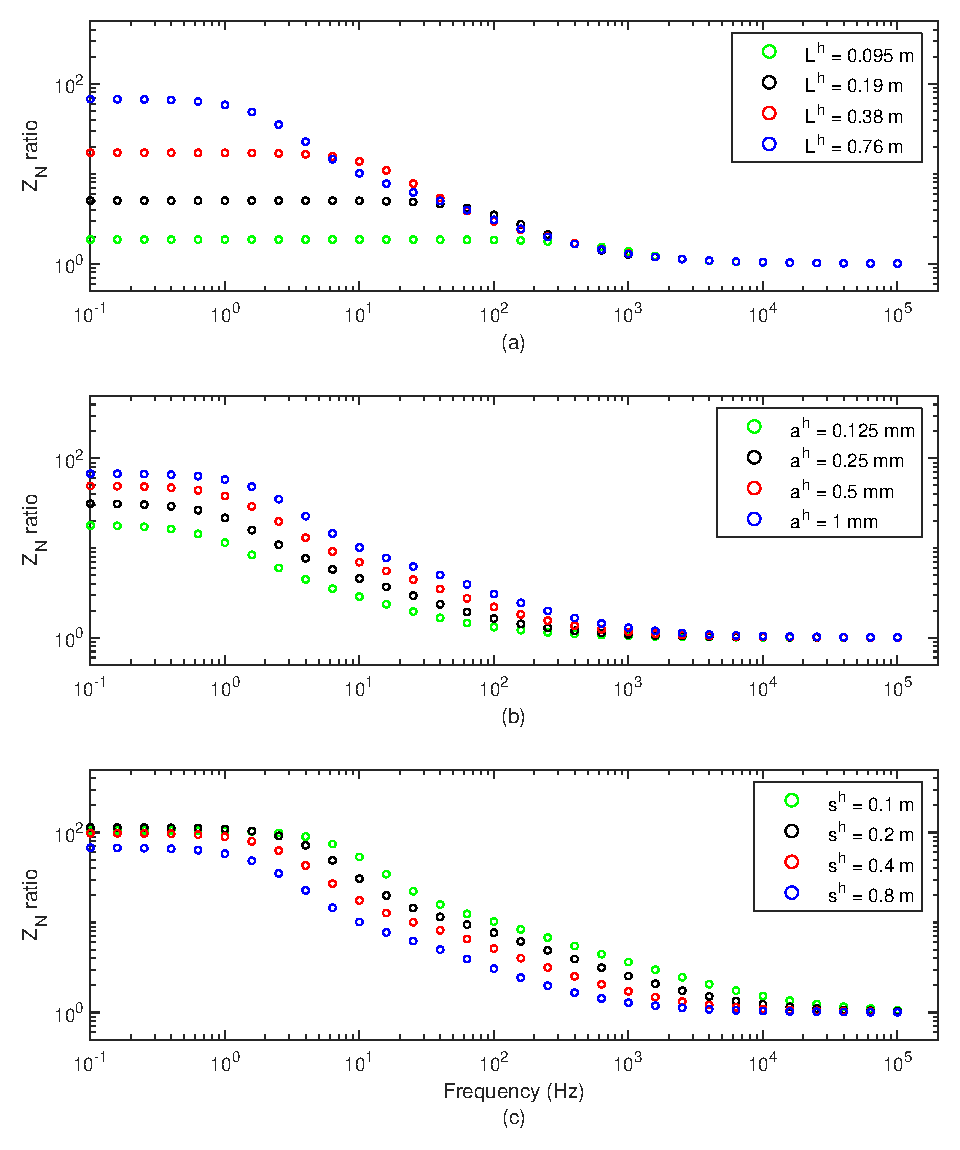
\includegraphics[ width=100mm, height=85mm]{sensitivityZN_geometry.eps}
\caption{
}
\label{fig.4}
\end{figure}

 \begin{figure}[!ht]
\centering
        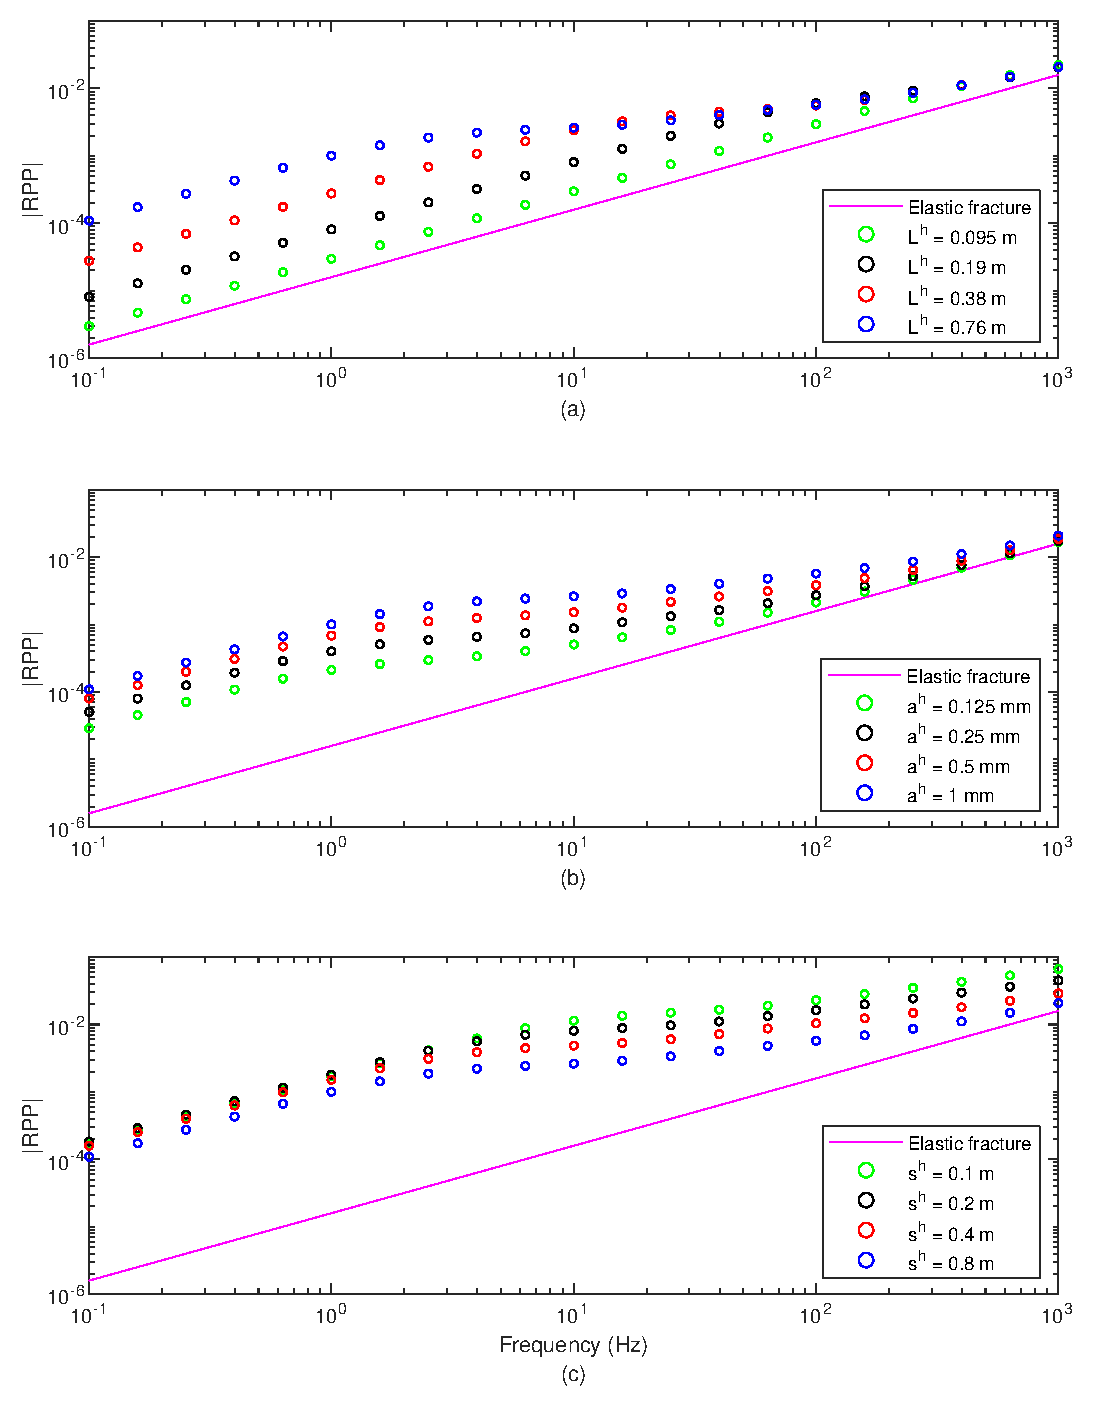
\includegraphics[ width=100mm, height=85mm]{sensitivityRPP_geometry.eps}
\caption{
}
\label{fig.5}
\end{figure}



\subsection{Sensitivity to secondary fracture physical and saturating fluid properties}

 \begin{figure}[!ht]
\centering
        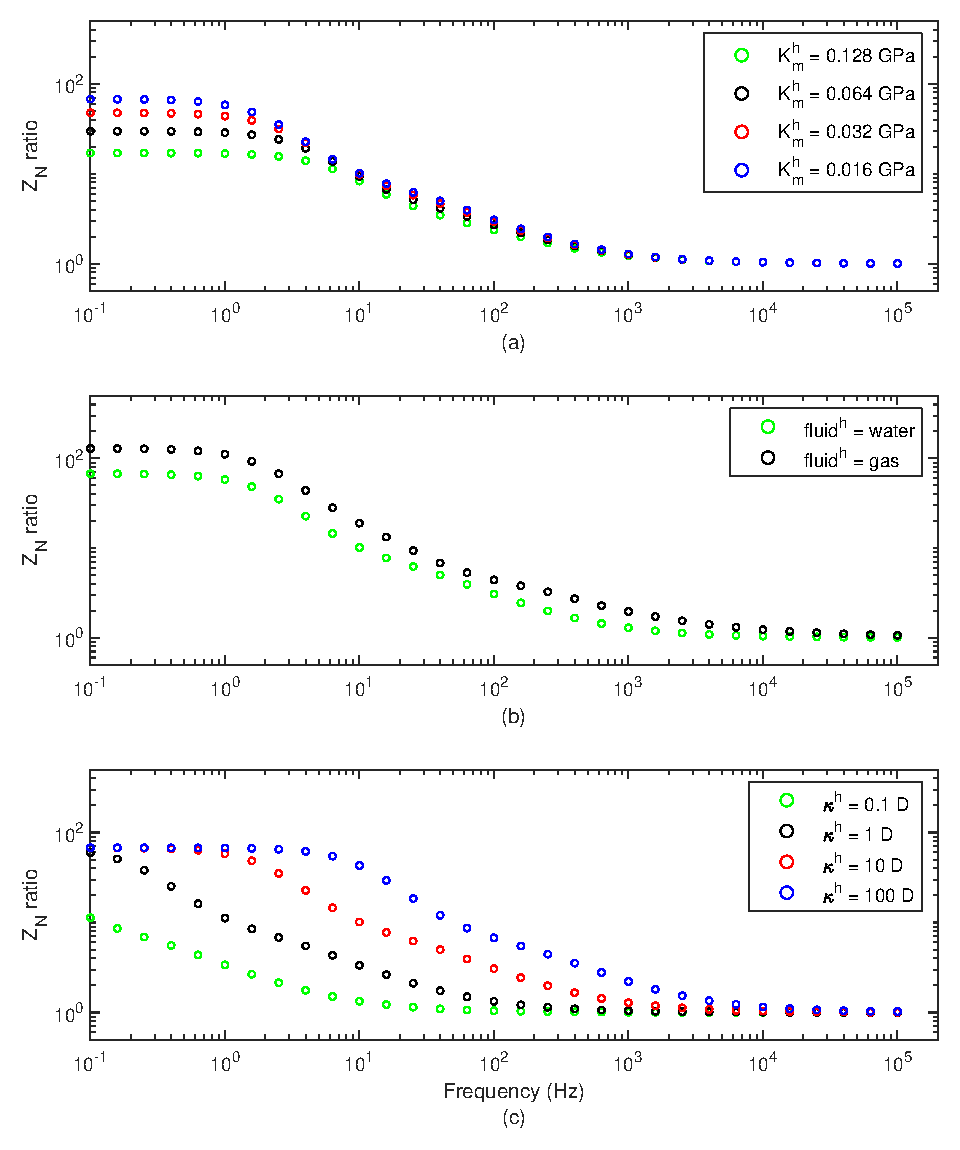
\includegraphics[ width=100mm, height=85mm]{sensitivityZN_physical.eps}
\caption{
}
\label{fig.6}
\end{figure}

 \begin{figure}[!ht]
\centering
        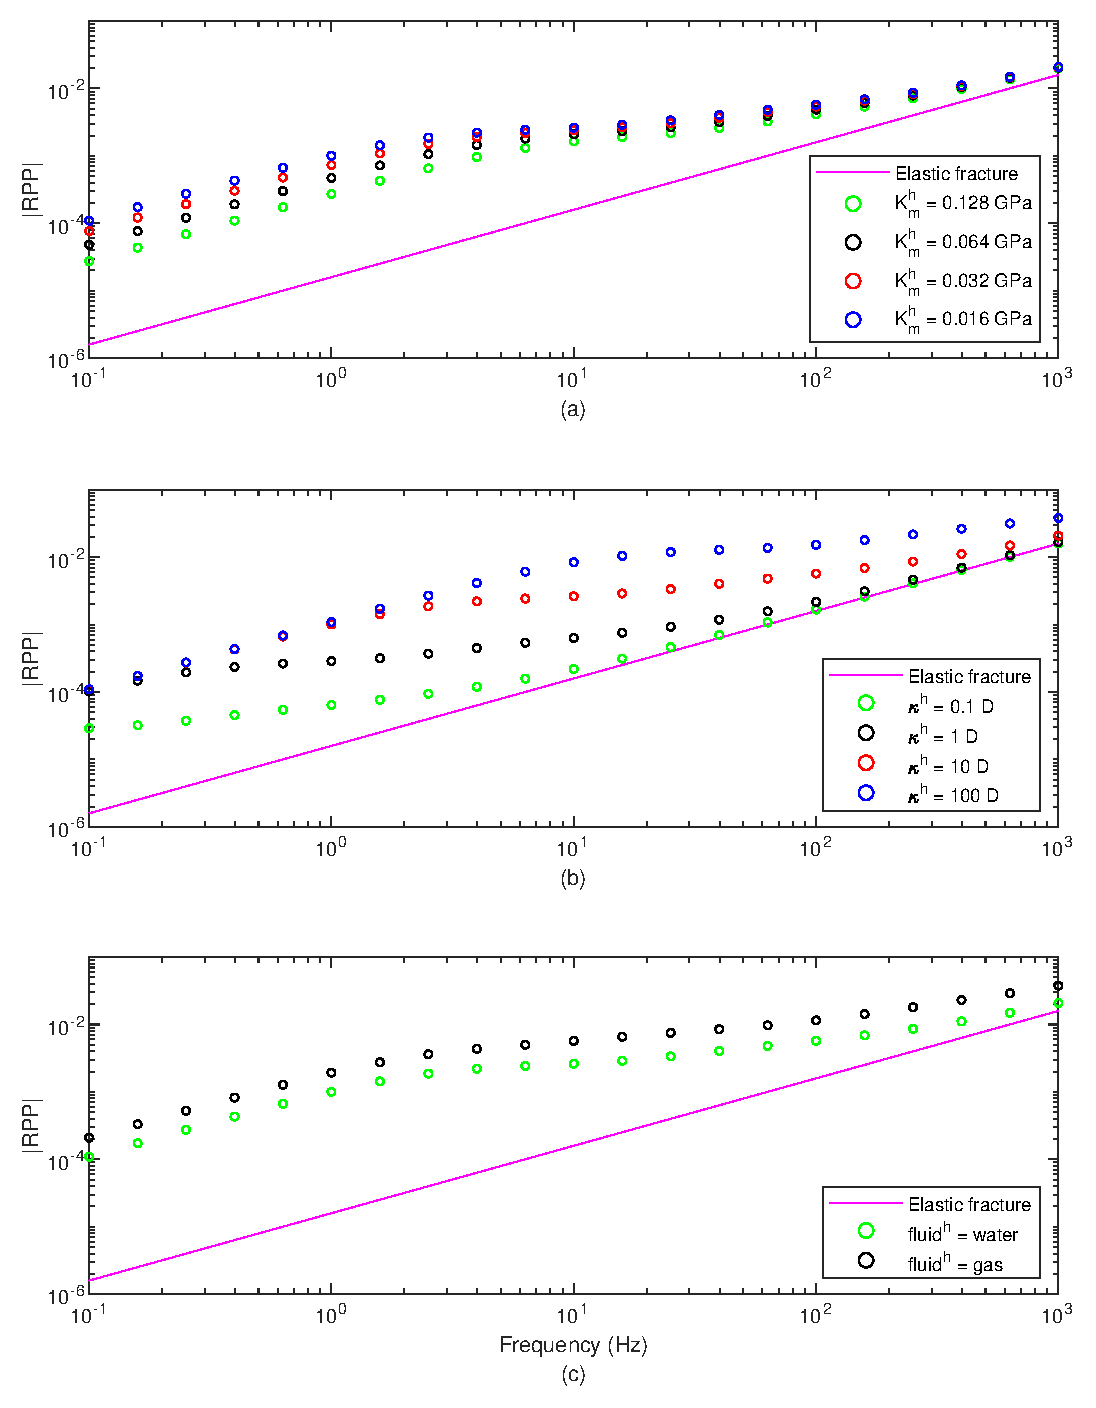
\includegraphics[ width=100mm, height=85mm]{sensitivityRPP_physical.eps}
\caption{
}
\label{fig.7}
\end{figure}


\section{Discussion}

\section{Conclusions}

%Text here ===>>>

%  To add line numbers to lines in equations,
%  \begin{linenomath*}
%  \begin{equation}
%  \end{equation}
%  \end{linenomath*}



%% Enter Figures and Tables near as possible to where they are first mentioned:
%
% DO NOT USE \psfrag or \subfigure commands.
%
% Figure captions go below the figure.
% Table titles go above tables;  other caption information
%  should be placed in last line of the table, using
% \multicolumn2l{$^a$ This is a table note.}
%
%----------------
% EXAMPLE FIGURES
%
% \begin{figure}
% \includegraphics{example.png}
% \caption{caption}
% \end{figure}
%
% Giving latex a width will help it to scale the figure properly. A simple trick is to use \textwidth. Try this if large figures run off the side of the page.
% \begin{figure}
% \noindent\includegraphics[width=\textwidth]{anothersample.png}
%\caption{caption}
%\label{pngfiguresample}
%\end{figure}
%
%
% If you get an error about an unknown bounding box, try specifying the width and height of the figure with the natwidth and natheight options. This is common when trying to add a PDF figure without pdflatex.
% \begin{figure}
% \noindent\includegraphics[natwidth=800px,natheight=600px]{samplefigure.pdf}
%\caption{caption}
%\label{pdffiguresample}
%\end{figure}
%
%
% PDFLatex does not seem to be able to process EPS figures. You may want to try the epstopdf package.
%

%
% ---------------
% EXAMPLE TABLE
% Please do NOT include vertical lines in tables
% if the paper is accepted, Wiley will replace vertical lines with white space
% the CLS file modifies table padding and vertical lines may not display well
%

%% SIDEWAYS FIGURE and TABLE
% AGU prefers the use of {sidewaystable} over {landscapetable} as it causes fewer problems.
%
% \begin{sidewaysfigure}
% \includegraphics[width=20pc]{figsamp}
% \caption{caption here}
% \label{newfig}
% \end{sidewaysfigure}
%
%  \begin{sidewaystable}
%  \caption{Caption here}
% \label{tab:signif_gap_clos}
%  \begin{tabular}{ccc}
% one&two&three\\
% four&five&six
%  \end{tabular}
%  \end{sidewaystable}

%% If using numbered lines, please surround equations with \begin{linenomath*}...\end{linenomath*}
%\begin{linenomath*}
%\begin{equation}
%y|{f} \sim g(m, \sigma),
%\end{equation}
%\end{linenomath*}

%%% End of body of article

%%%%%%%%%%%%%%%%%%%%%%%%%%%%%%%%
%% Optional Appendix goes here
%
% The \appendix command resets counters and redefines section heads
%
% After typing \appendix
%
%\section{Here Is Appendix Title}
% will show
% A: Here Is Appendix Title
%
\appendix
\section{Here is a sample appendix}

%%%%%%%%%%%%%%%%%%%%%%%%%%%%%%%%%%%%%%%%%%%%%%%%%%%%%%%%%%%%%%%%
%
% Optional Glossary, Notation or Acronym section goes here:
%
%%%%%%%%%%%%%%
% Glossary is only allowed in Reviews of Geophysics
%  \begin{glossary}
%  \term{Term}
%   Term Definition here
%  \term{Term}
%   Term Definition here
%  \term{Term}
%   Term Definition here
%  \end{glossary}

%
%%%%%%%%%%%%%%
% Acronyms
%   \begin{acronyms}
%   \acro{Acronym}
%   Definition here
%   \acro{EMOS}
%   Ensemble model output statistics
%   \acro{ECMWF}
%   Centre for Medium-Range Weather Forecasts
%   \end{acronyms}

%
%%%%%%%%%%%%%%
% Notation
%   \begin{notation}
%   \notation{$a+b$} Notation Definition here
%   \notation{$e=mc^2$}
%   Equation in German-born physicist Albert Einstein's theory of special
%  relativity that showed that the increased relativistic mass ($m$) of a
%  body comes from the energy of motion of the body—that is, its kinetic
%  energy ($E$)—divided by the speed of light squared ($c^2$).
%   \end{notation}



\section{Open Research}
AGU requires an Availability Statement for the underlying data needed to understand, evaluate, and build upon the reported research at the time of peer review and publication.

Authors should include an Availability Statement for the software that has a significant impact on the research. Details and templates are in the Availability Statement section of the Data and Software for Authors Guidance: \url{https://www.agu.org/Publish-with-AGU/Publish/Author-Resources/Data-and-Software-for-Authors#availability}

It is important to cite individual datasets in this section and, and they must be included in your bibliography. Please use the type field in your bibtex file to specify the type of data cited. Some options include Dataset, Software, Collection, ComputationalNotebook. Ex: 
\\
\begin{verbatim}

@misc{https://doi.org/10.7283/633e-1497,
  doi = {10.7283/633E-1497},
  url = {https://www.unavco.org/data/doi/10.7283/633E-1497},
  author = {de Zeeuw-van Dalfsen, Elske and Sleeman, Reinoud},
  title = {KNMI Dutch Antilles GPS Network - SAB1-St_Johns_Saba_NA P.S.},
  publisher = {UNAVCO, Inc.},
  year = {2019},
  type = {dataset}
}

\end{verbatim}

For physical samples, use the IGSN persistent identifier, see the International Geo Sample Numbers section:
\url{https://www.agu.org/Publish-with-AGU/Publish/Author-Resources/Data-and-Software-for-Authors#IGSN}
%%%%%%%%%%%%%%%%%%%%%%%%%%%%%%%%%%%%%%%%%%%%%%%

\acknowledgments
This section is optional. Include any Acknowledgments here.



%% ------------------------------------------------------------------------ %%
%% References and Citations

%%%%%%%%%%%%%%%%%%%%%%%%%%%%%%%%%%%%%%%%%%%%%%%
%
% \bibliography{<name of your .bib file>} don't specify the file extension
%
% don't specify bibliographystyle

% In the References section, cite the data/software described in the Availability Statement (this includes primary and processed data used for your research). For details on data/software citation as well as examples, see the Data & Software Citation section of the Data & Software for Authors guidance
% https://www.agu.org/Publish-with-AGU/Publish/Author-Resources/Data-and-Software-for-Authors#citation

%%%%%%%%%%%%%%%%%%%%%%%%%%%%%%%%%%%%%%%%%%%%%%%

\bibliography{reference}



%Reference citation instructions and examples:
%
% Please use ONLY \cite and \citeA for reference citations.
% \cite for parenthetical references
% ...as shown in recent studies (Simpson et al., 2019)
% \citeA for in-text citations
% ...Simpson et al. (2019) have shown...
%
%
%...as shown by \citeA{jskilby}.
%...as shown by \citeA{lewin76}, \citeA{carson86}, \citeA{bartoldy02}, and \citeA{rinaldi03}.
%...has been shown \cite{jskilbye}.
%...has been shown \cite{lewin76,carson86,bartoldy02,rinaldi03}.
%... \cite <i.e.>[]{lewin76,carson86,bartoldy02,rinaldi03}.
%...has been shown by \cite <e.g.,>[and others]{lewin76}.
%
% apacite uses < > for prenotes and [ ] for postnotes
% DO NOT use other cite commands (e.g., \citet, \citep, \citeyear, \citealp, etc.).
% \nocite is okay to use to add references from your Supporting Information
%



\end{document}



More Information and Advice:

%% ------------------------------------------------------------------------ %%
%
%  SECTION HEADS
%
%% ------------------------------------------------------------------------ %%

% Capitalize the first letter of each word (except for
% prepositions, conjunctions, and articles that are
% three or fewer letters).

% AGU follows standard outline style; therefore, there cannot be a section 1 without
% a section 2, or a section 2.3.1 without a section 2.3.2.
% Please make sure your section numbers are balanced.
% ---------------
% Level 1 head
%
% Use the \section{} command to identify level 1 heads;
% type the appropriate head wording between the curly
% brackets, as shown below.
%
%An example:
%\section{Level 1 Head: Introduction}
%
% ---------------
% Level 2 head
%
% Use the \subsection{} command to identify level 2 heads.
%An example:
%\subsection{Level 2 Head}
%
% ---------------
% Level 3 head
%
% Use the \subsubsection{} command to identify level 3 heads
%An example:
%\subsubsection{Level 3 Head}
%
%---------------
% Level 4 head
%
% Use the \subsubsubsection{} command to identify level 3 heads
% An example:
%\subsubsubsection{Level 4 Head} An example.
%
%% ------------------------------------------------------------------------ %%
%
%  IN-TEXT LISTS
%
%% ------------------------------------------------------------------------ %%
%
% Do not use bulleted lists; enumerated lists are okay.
% \begin{enumerate}
% \item
% \item
% \item
% \end{enumerate}
%
%% ------------------------------------------------------------------------ %%
%
%  EQUATIONS
%
%% ------------------------------------------------------------------------ %%

% Single-line equations are centered.
% Equation arrays will appear left-aligned.

Math coded inside display math mode \[ ...\]
 will not be numbered, e.g.,:
 \[ x^2=y^2 + z^2\]

 Math coded inside \begin{equation} and \end{equation} will
 be automatically numbered, e.g.,:
 \begin{equation}
 x^2=y^2 + z^2
 \end{equation}


% To create multiline equations, use the
% \begin{eqnarray} and \end{eqnarray} environment
% as demonstrated below.
\begin{eqnarray}
  x_{1} & = & (x - x_{0}) \cos \Theta \nonumber \\
        && + (y - y_{0}) \sin \Theta  \nonumber \\
  y_{1} & = & -(x - x_{0}) \sin \Theta \nonumber \\
        && + (y - y_{0}) \cos \Theta.
\end{eqnarray}

%If you don't want an equation number, use the star form:
%\begin{eqnarray*}...\end{eqnarray*}

% Break each line at a sign of operation
% (+, -, etc.) if possible, with the sign of operation
% on the new line.

% Indent second and subsequent lines to align with
% the first character following the equal sign on the
% first line.

% Use an \hspace{} command to insert horizontal space
% into your equation if necessary. Place an appropriate
% unit of measure between the curly braces, e.g.
% \hspace{1in}; you may have to experiment to achieve
% the correct amount of space.


%% ------------------------------------------------------------------------ %%
%
%  EQUATION NUMBERING: COUNTER
%
%% ------------------------------------------------------------------------ %%

% You may change equation numbering by resetting
% the equation counter or by explicitly numbering
% an equation.

% To explicitly number an equation, type \eqnum{}
% (with the desired number between the brackets)
% after the \begin{equation} or \begin{eqnarray}
% command.  The \eqnum{} command will affect only
% the equation it appears with; LaTeX will number
% any equations appearing later in the manuscript
% according to the equation counter.
%

% If you have a multiline equation that needs only
% one equation number, use a \nonumber command in
% front of the double backslashes (\\) as shown in
% the multiline equation above.

% If you are using line numbers, remember to surround
% equations with \begin{linenomath*}...\end{linenomath*}

%  To add line numbers to lines in equations:
%  \begin{linenomath*}
%  \begin{equation}
%  \end{equation}
%  \end{linenomath*}



